\subsection{Implementierung}

Zur Implementierung unseres REST-Services in Java verwenden wir Jersey \cite{Jersey}, die Standardbibliothek für Java-APIs für RESTful Services (JAX-RS). Jersey ermöglicht die Implementierung eines REST-Services innerhalb einer Java-Klasse, ohne die dabei notwendige HTML-Kommunikation explizit behandeln zu können. Wie bereits beschrieben, sind in einem REST-Service serverseitige Ressourcen definiert, mit denen ein Benutzer als Client über HTML-Anfragen an eine assoziierte URL interagieren kann.

Ein REST-Service funktioniert also immer in Reaktion auf eine Benutzer-Anfrage. Um diese Reaktion in Java implementieren zu können, kann in Jersey eine Ressource mit einer Java-Methode in Verbindung gesetzt werden. Das geschieht, indem für die Methode spezifiziert wird, welche Art von HTML-Anfrage auf welche URL zum Aufruf der Methode führt. Die URL setzt sich dabei aus den Einstellungen für die globale Basis-URL (welche gemeinsam mit anderen Einstellungen in einer \texttt{web.xml}-Datei festgelegt werden kann), dem URL-Bestandteil der Klasse und dem URL-Bestandteil der Methode zusammen. Die Bestandteile der Klasse und der Methode können dabei durch den Parameter der von Jersey bereitgestellten Annotation \texttt{@Path} definiert werden. Zusätzlich stehen außerdem Annotationen zur Verfügung, welche die Art der HTML-Anfrage spezifizieren, da jeweils unterschiedliche Methoden für ihre Ausführung notwendig sind. Von diesen haben wir ausschließlich \texttt{@GET} und \texttt{@POST} verwendet. Eine beispielhafte Verbindung der Methode \texttt{getTweets()} GET-Anfrage auf die URL \texttt{www.tmetrics.de/rest/tweets} (zusammengesetzt aus der Basis-URL \texttt{www.tmetrics.de} sowie den Bestandteilen \texttt{/rest} der Klasse und \texttt{/tweets} der Methode) ist in Abbildung \ref{jerseyurl} zu sehen.

\begin{figure}[h]
\centering
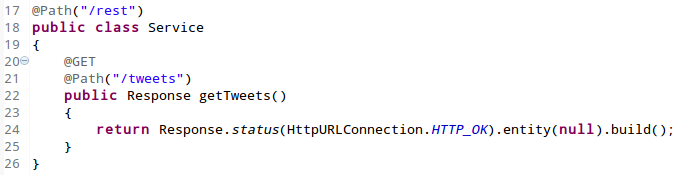
\includegraphics[scale=0.6]{Bilder/REST/JerseyURL.png}
\caption{Jersey: Verbindung von Methoden mit HTML-Anfragen}
\label{jerseyurl}
\end{figure}

Wie ebenfalls an der Abbildung erkennbar ist, liefert jede mit Jersey implementierte Methode eines REST-Servers standardmäßig eine HTML-Response zurück, welche durch die \texttt{Response}-Klasse repräsentiert wird. Die eigentlichen Antwortdaten können dabei als Bestandteil des Entity-Attributs der Response übergeben werden (in diesem Beispiel nur \texttt{null}). Dabei kann mit einer weiteren Annotation spezifiziert werden, in welcher Form die Daten in der Entity an das Frontend gesendet werden. Da das Frontend in JavaScript implementiert ist, haben wir uns hier für das auf JavaScript ausgerichtete JSON-Format entschieden. Dieses kann über den Parameter der Annotation \texttt{@Produces} spezifiziert werden (siehe Abbildung \ref{jerseyproduces}). Primitive Datentypen sowie in JavaScript vorhandene Datenstrukturen werden dabei automatisch geparst. Für eigene Klassen muss das Parsing explizit definiert werden (siehe Abschnitt \ref{sec:dto}). Dieses Parsing macht es sogar möglich, anstatt einer expliziten Response direkt die Daten zurückzugeben. Diese werden dann implizit in eine Response verpackt. Dieses Vorgehen wurde zeitweise von uns eingesetzt, aber im Projektverlauf verworfen, da uns eine explizite Kontrolle der Response insbesondere wegen der Statusnachricht als sinnvoll erschien.

\begin{figure}[h]
\centering
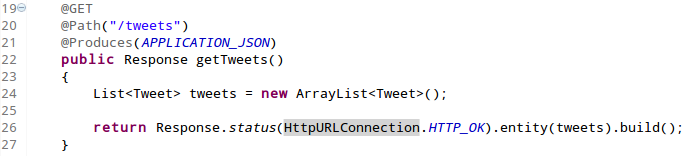
\includegraphics[scale=0.6]{Bilder/REST/JerseyProduces.png}
\caption{Jersey: Spezifizierung des Rückgabeformats}
\label{jerseyproduces}
\end{figure}

Häufig ist außerdem der Zugriff nur auf bestimmte Bestandteile einer Ressource notwendig. So ist niemals der gesamte Inhalt der Tweets-Ressource von Interesse, sondern nur die Tweets, die mit einem bestimmten Suchbegriff verbunden sind (welcher durch eine ID identifiziert wird). Es sind außerdem weitere Einschränkungen der Daten vorstellbar. So sind in bestimmten Ansichten nur Tweets aus einem bestimmtem Zeitraum oder mit einem bestimmten Sentiment von Interesse. Diese Parameter finden sich einerseits als Parameter in der URL der HTML-Anfrage und andererseits in der Signatur der entsprechenden Java-Methode wieder. Die Jersey-Annotation \texttt{@QueryParam} ermöglicht dabei die Verbindung eines Parameters der Anfrage mit einem Argument in der Methodensignatur. Dabei ist zu beachten, dass sämtliche Argumente \texttt{null} sind, falls ihnen entweder im Quellcode kein Anfrageparameter zugewiesen wurde oder falls die Anfrage diesen Parameter nicht beinhaltet. Soll also ein Parameter verpflichtend gemacht werden, muss diese Situation abgefangen und eine Exception geworfen werden. Eine Alternative bildet die Verwendung der Annotation \texttt{@DefaultValue}, womit ein Standardwert festgelegt wird, falls der Parameter nicht in der Anfrage vorkommt. Eine genauere Behandlung dieser Fälle wird in Abschnitt \ref{sec:serviceklassen} beschrieben. Auf ähnliche Weise können Methodenargumente über die Annotation \texttt{@HeaderParam} auch auf die Header-Parameter der HTML-Anfrage zugreifen. Diese Fälle werden in Abbildung \ref{jerseyparams} veranschaulicht. Ein valider Zugriff auf die in dieser Methode spezifizierte Ressource wäre beispielsweise eine GET-Anfrage auf \texttt{www.tmetrics.de/rest/tweets?id=1\&limit=100}. Aufgrund des Standardwertes könnte der \texttt{limit}-Parameter dabei auch weggelassen werden.

\begin{figure}[h]
\centering
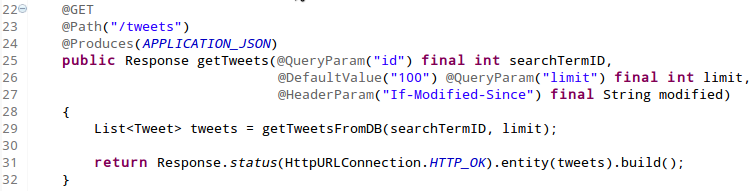
\includegraphics[scale=0.6]{Bilder/REST/JerseyParams.png}
\caption{Jersey: Übergabe von Parametern}
\label{jerseyparams}
\end{figure}

Auf diese Weise ermöglicht Jersey es, Java-Methoden mit HTML-Anfragen auf eine URL zu verknüpfen und die Eingaben und Ausgaben dieser Methode zu kontrollieren. Um eine konkrete HTML-Anfrage abzuhandeln, wird die Klasse, in der Jersey implementiert ist, neu instanziiert und die korrekte Methode identifiziert und ausgeführt. Diese neuerliche Instanziierung bei jeder Anfrage spiegelt die Tatsache wieder, dass ein REST-Service zustandslos ist.